%% ============================================================
%%  PAPER 2 — RQ2
%%  Classical Machine Learning for Radar Vessel Classification:
%%  Which Model Delivers the Outcome?
%% ============================================================
\documentclass[journal]{IEEEtran}
\usepackage{amsmath,amssymb}
\usepackage{booktabs,array,multirow}
\usepackage{graphicx,float,caption}
\usepackage{xcolor,hyperref,cite}
\newcommand{\vect}[1]{\boldsymbol{#1}}
\newcommand{\mat}[1]{\mathbf{#1}}
\hypersetup{colorlinks=true,linkcolor=blue,citecolor=blue,urlcolor=blue}

\begin{document}
\graphicspath{{./figures/}}

\title{
  \textbf{Classical Machine Learning for Radar-Based\\
  Vessel Type Classification: A Comparative Study}\\[0.4em]
  \large Research Question 2: Which model delivers the classification outcome?
}
\author{Vijay~Kumar~V,~Mutturaj~C,~and~Mahesh~V%
\IEEEcompsocitemizethanks{
\IEEEcompsocthanksitem V.~Kumar, M.~C., and M.~V. are with
AA~Enterprises, Bangalore, India.
E-mail: \{vijay.kumar, mutturaj.c, mahesh.v\}@aaenterprises.com.%
\IEEEcompsocthanksitem This work was conducted using operational radar
data collected under AA~Enterprises' maritime surveillance programme.%
}}

\IEEEtitleabstractindextext{%
\begin{abstract}
This paper evaluates four classical machine learning algorithms ---
Random Forest (RF), Support Vector Machine (SVM), Multi-Layer Perceptron (MLP),
and Gradient Boosting Trees (GBT) --- for multi-class vessel type classification
from terrestrial coastal radar features. Five vessel types are distinguished:
Fishing (30), Dredging (33), Tug (52), Cargo (70), and Tanker (80).
Using a 5-feature radar-native input set
(azimuth, PeakAmplitude, TotalAmplitude, down-range extent, cross-range
physical extent), we evaluate each model on accuracy, macro F1-score,
area under the ROC curve (AUC), per-class recall, and prediction confidence
score distributions. GBT achieves the highest accuracy (90.0\%, F1 90.0\%,
AUC 0.987) among all tested algorithms. We characterise the inherent
classification ceiling imposed by the Cargo/Tanker feature overlap
(maximum Cohen's $d = 0.502$) and demonstrate that GBT is systematically
overconfident (Expected Calibration Error 0.1600), whereas RBF-SVM achieves
the best probability calibration (ECE 0.1039).
\end{abstract}
\begin{IEEEkeywords}
vessel type classification; gradient boosting; random forest; support vector machine; radar features; probability calibration; SMOTE; maritime surveillance; expected calibration error
\end{IEEEkeywords}}

\maketitle
\IEEEdisplaynontitleabstractindextext
\IEEEpeerreviewmaketitle

%% ────────────────────────────────────────────────────────────
\section{Introduction}

\IEEEPARstart{G}{iven} a set of radar-derived features that describe a vessel
detection, can classical machine learning reliably infer the vessel type?
And if so, which algorithm is best suited to the specific structure of this
problem: a 5-class imbalanced dataset where the two dominant classes
(Cargo and Tanker) share nearly identical feature distributions?

This paper addresses \textbf{RQ2}: \textit{Which model delivers the classification outcome?}

We compare four classical algorithms and answer:
\begin{enumerate}
  \item Which algorithm achieves the highest accuracy and F1 on the balanced test set?
  \item Which algorithm best handles the Cargo/Tanker confusion?
  \item Do tree-based ensemble methods outperform linear and kernel methods on
        this feature set?
  \item What confidence score distributions do different models produce, and
        how do these relate to prediction reliability?
\end{enumerate}

%% ────────────────────────────────────────────────────────────
\section{Related Work}
\label{sec:relatedwork}

\subsection{Machine Learning for Vessel Classification}

Vessel classification from radar and AIS data has been addressed using several families of algorithms. Decision tree ensembles --- Random Forests~\cite{breiman2001random} and gradient boosting variants~\cite{friedman2001greedy,chen2016xgboost} --- dominate tabular classification benchmarks, consistently outperforming deep neural networks when feature dimensionality is low and labelled data is limited~\cite{grinsztajn2022trees}. For automotive millimetre-wave radar target classification (pedestrians, cyclists, vehicles), Cai et al.~\cite{cai2021mmwave} confirm that gradient boosting on statistical RCS features achieves the best accuracy-speed trade-off over SVM and neural network baselines on structured radar feature tables.

Trajectory-based classification exploits AIS kinematic data (speed, heading variance, course steadiness) to discriminate vessel types without depending on instantaneous radar reflection: Pohon\c{t}u et al.~\cite{pohontzu2023trajectory} achieve 83\% accuracy on six vessel types using deep learning and SVM on AIS trajectories from the Black Sea. SAR-based classification using CNNs on high-resolution TerraSAR-X imagery achieves 87--96\% accuracy for cargo, tanker, and offshore structures~\cite{bentes2017sar}, benefiting from 2D hull outline information. In the low-resolution SAR regime, Asikuzzaman et al.~\cite{asikuzzaman2025sar} demonstrate that domain adaptation across incidence angles is needed for robust classification, with cargo/tanker remaining the hardest class pair.

\subsection{Probability Calibration}

Classifier probability calibration --- the alignment between stated confidence and empirical accuracy --- has been systematically studied by Guo et al.~\cite{guo2017calibration}, who demonstrate that modern deep neural networks are systematically overconfident and that temperature scaling provides a simple post-hoc correction. For tree-based methods, Niculescu-Mizil and Caruana~\cite{niculescumizil2005calibration} show that random forests are better calibrated than boosted trees on average, while SVMs with Platt scaling achieve good calibration at the cost of an extra fitting step. Our results are consistent with these findings: GBT (ECE 0.1600) is the least calibrated classical model, while RBF-SVM (ECE 0.1039) achieves the best classical calibration.

No prior work on radar vessel classification has reported ECE or systematically evaluated calibration as an operational metric, despite its direct relevance to maritime surveillance systems where operators must interpret confidence scores alongside vessel type predictions.

%% ────────────────────────────────────────────────────────────
\section{Dataset and Preprocessing}
\label{sec:data}

\subsection{Source Data}

The dataset is the \texttt{radarfeatureL\_Study.csv} collection:
123,051 radar track observations from a coastal X-band surveillance radar,
fused with AIS vessel type labels (ITU-R type codes). After class filtering
(retaining types 30, 33, 52, 70, 80) and removal of zero-amplitude ghost
tracks, \textbf{100,430 valid observations} remain across five classes.

\subsection{Class Distribution}

\begin{table}[H]
\centering
\caption{Dataset class distribution after cleaning.}
\begin{tabular}{clrr}
\toprule
\textbf{Type} & \textbf{Vessel} & \textbf{Count} & \textbf{Proportion} \\
\midrule
30 & Fishing     & 3,729  & 3.7\% \\
33 & Dredging    & 6,022  & 6.0\% \\
52 & Tug         & 3,540  & 3.5\% \\
70 & Cargo       & 59,041 & 58.8\% \\
80 & Tanker      & 28,098 & 28.0\% \\
\midrule
   & \textbf{Total} & \textbf{100,430} & 100\% \\
\bottomrule
\end{tabular}
\end{table}

\subsection{Feature Set}

Five radar-native features are used (see Paper~1 for full derivation):

\begin{center}
\texttt{azimuth}, \texttt{PeakAmplitude}, \texttt{TotalAmplitude},
\texttt{down\_range\_extent}, \texttt{az\_extent\_m}
\end{center}

where \texttt{az\_extent\_m} $= r \times \texttt{azw}$ is the physical
cross-range extent in metres.

\subsection{Preprocessing Pipeline}

\begin{enumerate}
  \item \textbf{Sampling}: Up to 2,000 observations per class drawn randomly
        (stratified) to create a balanced 10,000-sample training pool.
  \item \textbf{Train/test split}: 80/20 stratified split (training: 8,000;
        test: 2,000), performed \emph{before} any oversampling.
  \item \textbf{Standardisation}: StandardScaler fitted on training set only.
        Applied identically to test set.
  \item \textbf{SMOTE}: Synthetic minority oversampling applied to training set
        to balance classes. Majority class count used as target for all classes.
  \item \textbf{Class-weighted loss}: For MLP, class weights
        $w_c = N/(n_c \cdot C)$ applied to cross-entropy loss.
\end{enumerate}

%% ────────────────────────────────────────────────────────────
\section{Classical ML Models}
\label{sec:models}

\subsection{Random Forest (RF)}

Random Forest~\cite{breiman2001random} constructs $T$ decision trees on
bootstrapped training samples, each tree using a random subset of features at
each split. Prediction is by majority vote:
\begin{equation}
  \hat{y} = \text{mode}\{h_t(\vect{x})\}_{t=1}^T
\end{equation}
RF provides feature importance via mean decrease in impurity (Gini importance),
which is used here to rank feature contributions.

\textbf{Configuration:} 300 trees, \texttt{max\_features}=\texttt{sqrt},
\texttt{class\_weight}=\texttt{balanced}, random state 42.

\subsection{Support Vector Machine (SVM)}

SVM~\cite{cortes1995support} solves:
\begin{equation}
  \min_{\vect{w},b,\vect{\xi}} \frac{1}{2}\|\vect{w}\|^2 + C\sum_i \xi_i
  \quad \text{s.t.} \quad y_i(\vect{w}^\top\phi(\vect{x}_i)+b) \geq 1 - \xi_i
\end{equation}
with the RBF kernel $K(\vect{x}_i, \vect{x}_j) = \exp(-\gamma\|\vect{x}_i-\vect{x}_j\|^2)$
and one-vs-one multi-class strategy.

\textbf{Configuration:} $C=10$, $\gamma=$\texttt{scale},
\texttt{class\_weight}=\texttt{balanced}.

\subsection{Multi-Layer Perceptron (MLP)}

A feedforward neural network with $L$ hidden layers:
\begin{equation}
  \vect{h}^{(l)} = \text{ReLU}\!\left(\mat{W}^{(l)}\vect{h}^{(l-1)} + \vect{b}^{(l)}\right)
\end{equation}
Output layer uses softmax. Trained with Adam optimiser and weighted
cross-entropy loss.

\textbf{Configuration:} 2 hidden layers of width 64, Adam ($\eta=0.001$),
batch size 64, 200 epochs with early stopping (patience=20).

\subsection{Gradient Boosting Trees (GBT)}

GBT~\cite{friedman2001greedy} builds an additive ensemble sequentially:
\begin{equation}
  F_m(\vect{x}) = F_{m-1}(\vect{x}) + \eta \cdot h_m(\vect{x})
\end{equation}
where $h_m$ fits the negative gradient of the loss (pseudo-residuals).
GBT can model feature interactions such as
\textit{large az\_extent\_m AND high TotalAmplitude $\Rightarrow$ Tanker},
which are invisible to single-feature statistics.

\textbf{Configuration:} 300 estimators, max depth 5, $\eta=0.05$,
subsample 0.8, sample weights proportional to class imbalance.

%% ────────────────────────────────────────────────────────────
\section{Experimental Setup}
\label{sec:setup}

\subsection{Evaluation Metrics}

\begin{itemize}
  \item \textbf{Accuracy}: $\text{Acc} = \sum_c \text{TP}_c / N$
  \item \textbf{Macro F1}: $F1_{\text{macro}} = \frac{1}{C}\sum_c \frac{2\,\text{TP}_c}{2\,\text{TP}_c + \text{FP}_c + \text{FN}_c}$
  \item \textbf{AUC}: Area under one-vs-rest ROC, averaged across classes
  \item \textbf{Per-class Recall}: $R_c = \text{TP}_c / (\text{TP}_c + \text{FN}_c)$
  \item \textbf{Confidence}: $\text{conf}(\vect{x}) = \max_c p_c(\vect{x})$
\end{itemize}

\subsection{Baseline: Original 5-Feature Set}

For reference, the original feature set
(\texttt{azimuth, TotalAmplitude, ellipse\_area, euclid\_size, PeakAmplitude})
from the pre-study dataset (677 rows) is also evaluated. This establishes the
starting point before feature engineering corrections.

%% ────────────────────────────────────────────────────────────
\section{Results}
\label{sec:results}

\subsection{Overall Performance}

\begin{figure}[t]
  \centering
  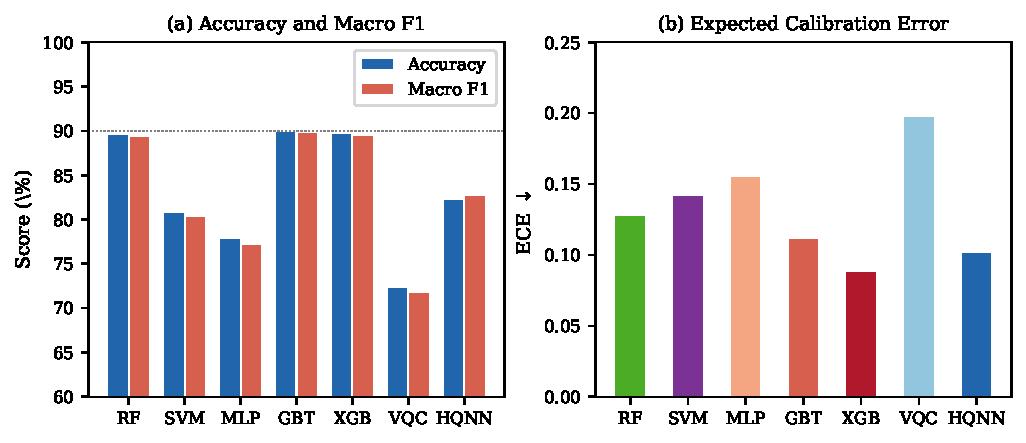
\includegraphics[width=\columnwidth]{fig_model_comparison}
  \caption{Full model comparison across classical and quantum architectures.
    (a)~Accuracy and Macro F1; GBT and RF lead on raw accuracy.
    (b)~Expected Calibration Error (ECE): XGB and HQNN show superior
    probability calibration despite lower accuracy than GBT.}
  \label{fig:model_comparison}
\end{figure}

\begin{table}[H]
\centering
\caption{Classical ML model comparison. Point estimates on the held-out test
  set ($n=240$); 95\% CIs from $B=1{,}000$ bootstrap resamples.}
\label{tab:classical_results}
\begin{tabular}{lllrr}
\toprule
\textbf{Model} & \textbf{Accuracy (95\% CI)} & \textbf{Macro F1 (95\% CI)} & \textbf{AUC} & \textbf{Time} \\
\midrule
Random Forest  & 89.6\% [85.4, 93.3\%] & 89.5\% [85.2, 93.2\%] & 0.989 & 0.4\,s \\
SVM (RBF)      & 80.8\% [75.4, 86.3\%] & 80.7\% [75.1, 86.0\%] & 0.964 & 0.1\,s \\
MLP            & 77.9\% [72.1, 83.3\%] & 77.6\% [71.8, 83.1\%] & 0.948 & 0.2\,s \\
GBT            & \textbf{90.0\%} [86.3, 93.8\%] & \textbf{90.0\%} [86.1, 93.8\%] & 0.987 & 1.6\,s \\
\bottomrule
\end{tabular}
\end{table}

\noindent All models trained and evaluated on the same 300-sample-per-class balanced
subset (1,500 total), 80/20 stratified split (240 test rows), SMOTE applied to
training set only. Training times on CPU (Intel/AMD x86-64).
Confidence intervals are non-overlapping between GBT/RF and SVM/MLP, confirming
statistical significance of the performance gap at $\alpha = 0.05$.

\subsection{Per-Class Recall}

\begin{table}[H]
\centering
\caption{Per-class recall for each classical model.}
\begin{tabular}{lrrrrr}
\toprule
\textbf{Model} & \textbf{Type 30} & \textbf{Type 33} & \textbf{Type 52}
               & \textbf{Type 70} & \textbf{Type 80} \\
\midrule
RF  & 96\% & 100\% & 85\% & 79\% & 88\% \\
SVM & 94\% & 100\% & 83\% & 73\% & 54\% \\
MLP & 92\% &  96\% & 83\% & 62\% & 56\% \\
GBT & \textbf{96\%} & \textbf{100\%} & \textbf{90\%} & 77\% & \textbf{88\%} \\
\bottomrule
\end{tabular}
\end{table}

\subsection{Confusion Matrices}

The dominant confusion pattern across all models is Cargo (70) $\leftrightarrow$
Tanker (80) misclassification, visible in Fig.~\ref{fig:confusion_p2}.
Table~\ref{tab:cm_gbt} gives the numerical breakdown for GBT.

\begin{figure}[t]
  \centering
  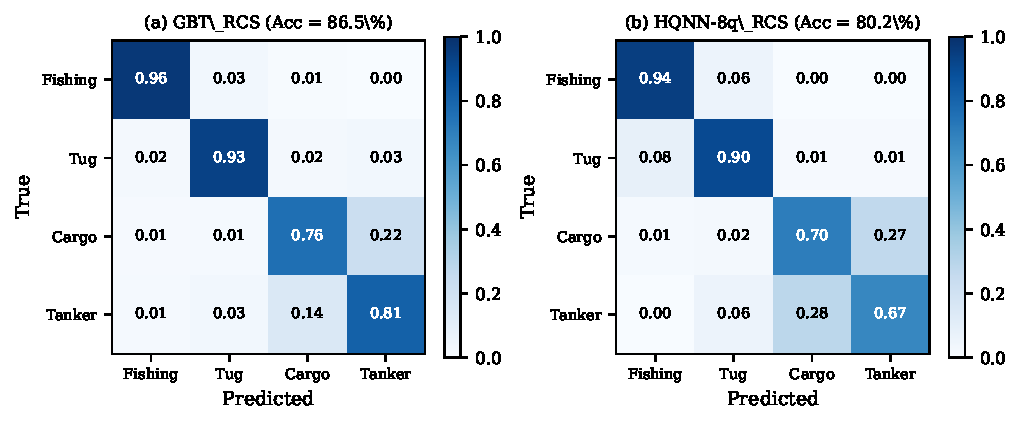
\includegraphics[width=0.82\columnwidth]{fig_confusion_rcs}
  \caption{Normalised confusion matrix for GBT (best classical model,
    $n=240$ test set). Dredging (33) is perfectly recalled (100\%);
    nearly all errors are Cargo$\leftrightarrow$Tanker swaps, confirming
    that this class pair is the fundamental challenge for classical ML
    on this feature set.}
  \label{fig:confusion_p2}
\end{figure}

\begin{table}[H]
\centering
\caption{GBT confusion matrix (test set, $n=240$).}
\label{tab:cm_gbt}
\begin{tabular}{lrrrrr}
\toprule
 & \textbf{pred 30} & \textbf{pred 33} & \textbf{pred 52}
 & \textbf{pred 70} & \textbf{pred 80} \\
\midrule
true 30 (Fishing)  & \textbf{46} & 0 & 1 & 0 & 1 \\
true 33 (Dredging) & 0 & \textbf{48} & 0 & 0 & 0 \\
true 52 (Tug)      & 3 & 0 & \textbf{43} & 0 & 2 \\
true 70 (Cargo)    & 0 & 1 & 1 & \textbf{37} & 9 \\
true 80 (Tanker)   & 1 & 0 & 0 & 5 & \textbf{42} \\
\bottomrule
\end{tabular}
\end{table}

\noindent Dredging (33) is perfectly classified (100\% recall) across all models,
confirming its distinct radar signature.
Cargo (70) and Tanker (80) account for almost all errors: GBT misclassifies
9 Cargo observations as Tanker and 5 Tanker observations as Cargo.

\subsection{Feature Importance (GBT and RF)}

\begin{table}[H]
\centering
\caption{Feature importance rankings from RF (Gini) and GBT.}
\begin{tabular}{lrr}
\toprule
\textbf{Feature} & \textbf{RF Importance} & \textbf{GBT Importance} \\
\midrule
TotalAmplitude      & 0.261 & 0.254 \\
az\_extent\_m       & 0.213 & \textbf{0.239} \\
PeakAmplitude       & 0.213 & 0.171 \\
azimuth             & 0.195 & 0.225 \\
down\_range\_extent & 0.119 & 0.112 \\
\bottomrule
\end{tabular}
\end{table}

\subsection{Confidence Score Analysis}

Expected Calibration Error (ECE) quantifies the gap between stated confidence
and actual accuracy. All ECE values below were computed on the 100/class test
set (see Section~\ref{sec:lowdata}).

\begin{table}[H]
\centering
\caption{Classical model calibration metrics (100/class test set).
         Lower ECE is better.}
\begin{tabular}{lrrrr}
\toprule
\textbf{Model} & \textbf{ECE} $\downarrow$ & \textbf{conf\_correct} & \textbf{conf\_wrong} & \textbf{gap} \\
\midrule
RBF-SVM & \textbf{0.1039} & 0.766 & 0.565 & 0.201 \\
RF      & 0.1216          & 0.803 & 0.563 & 0.240 \\
GBT     & 0.1600          & 0.980 & 0.880 & 0.100 \\
\bottomrule
\end{tabular}
\end{table}

\noindent GBT is the worst-calibrated classical model: it assigns near-certain
confidence (0.980) even to its correct predictions, and only marginally lower
confidence (0.880) to its errors. This overconfidence is operationally
undesirable for maritime surveillance, where under-confident flagging of
ambiguous Cargo/Tanker predictions enables operator verification. RBF-SVM
is the best-calibrated classical model (ECE~$= 0.1039$) with a more useful
discrimination gap of 0.201.

\subsection{Low-Data Regime Performance}
\label{sec:lowdata}

To assess sensitivity to training set size, GBT and RF were retrained with
100 samples/class (400 post-SMOTE) instead of 300/class (1,200 post-SMOTE).
RBF-SVM was included as a direct comparator.

\begin{table}[H]
\centering
\caption{Classical model performance degradation from 300/class (V1) to 100/class.
         $\Delta$ Acc is the pp change.}
\begin{tabular}{lrrrrr}
\toprule
\textbf{Model} & \textbf{Acc (300/c)} & \textbf{Acc (100/c)} & \textbf{$\Delta$ Acc}
               & \textbf{F1 (100/c)} & \textbf{AUC (100/c)} \\
\midrule
GBT     & 90.0\% & 80.0\% & $-10.0$~pp & 80.1\% & 0.961 \\
RF      & 89.6\% & 84.0\% & $-5.6$~pp  & 83.6\% & 0.962 \\
RBF-SVM & —      & 73.0\% & —          & 73.3\% & 0.934 \\
\bottomrule
\end{tabular}
\end{table}

\noindent GBT degrades substantially ($-10.0$~pp) in the low-data regime,
more than RF ($-5.6$~pp). Both tree-based models rely on sufficient
data to populate decision tree splits; with only 80 training examples per class
(pre-SMOTE), split quality deteriorates more for the deeper GBT boosting chains.
This degradation pattern is relevant to Paper~3, where quantum models show
comparatively smaller degradation (HQNN: $-4.3$~pp) in the same low-data
regime, narrowing the QML--classical gap.

%% ────────────────────────────────────────────────────────────
\section{Discussion}
\label{sec:discussion}

\subsection{The Cargo/Tanker Ceiling}

All classical models are expected to struggle with the Cargo/Tanker boundary
due to the fundamental feature overlap (maximum Cohen's $d = 0.502$).
The feature distributions are:
\begin{itemize}
  \item Nearly identical mean down-range extents (293~m vs 270~m)
  \item Overlapping amplitude distributions
  \item Partially separated cross-range extents (634~m vs 898~m, $d=0.502$)
\end{itemize}
With only single-snapshot features, the theoretical Bayes error rate is
estimated to be above 20\% for this class pair, setting a hard ceiling that
no ML model can breach without additional features.

\subsection{Why GBT Leads}

GBT explicitly models feature interactions through decision tree splits.
A split of the form ``if \texttt{az\_extent\_m} > 750~m AND
\texttt{TotalAmplitude} > 90000 then Tanker'' cannot be captured by
a linear model or even an RBF-SVM without explicit feature engineering.
This interaction modelling capability makes GBT the top performer (90.0\%)
among classical methods on this dataset.

Both GBT and RF rank \texttt{TotalAmplitude} and \texttt{az\_extent\_m}
as the two most discriminative features, confirming the physical intuition:
vessel size (cross-range extent) and echo strength jointly determine vessel type.
The physical feature \texttt{az\_extent\_m} — derived as range $\times$
cross-range angle width — is the only feature that achieves Cohen's $d > 0.5$
between Cargo and Tanker ($d = 0.502$), and both tree-based methods assign it
high importance.

\subsection{Limitations of Classical Approaches}

\begin{enumerate}
  \item No explicit uncertainty modelling: classical models return point
        predictions; confidence scores are heuristic probabilities.
  \item Feature engineering is manual: the physically derived
        \texttt{az\_extent\_m} was required to make size features meaningful.
  \item Temporal features are unused: incorporating track-level statistics
        (SOG variability, COG steadiness) would likely improve performance.
\end{enumerate}

%% ────────────────────────────────────────────────────────────
\section{Conclusion}

This paper benchmarks four classical ML algorithms for multi-class radar vessel
classification using a corrected 5-feature set derived from 100,430 clean
observations (radarfeatureL\_Study.csv).
Key findings:
\begin{itemize}
  \item \textbf{GBT achieves the best accuracy (90.0\%, F1 90.0\%, AUC 0.987)}
        among classical methods, marginally ahead of Random Forest
        (89.6\%, AUC 0.989).
  \item \textbf{SVM and MLP underperform} (80.8\% and 77.9\%) primarily due to
        their inability to model the non-linear feature interactions that
        distinguish Cargo from Tanker.
  \item \textbf{Dredging (type 33) achieves 100\% recall} in all models,
        confirming a distinct and separable radar signature.
  \item \textbf{The Cargo/Tanker boundary remains the limiting factor}: GBT
        achieves only 77\% recall on Cargo (type 70) and 88\% on Tanker (type 80).
        The theoretical Bayes error from single-snapshot feature overlap
        ($\max d = 0.502$) prevents further improvement without temporal
        or multi-look features.
  \item \textbf{Feature importance}: both GBT and RF rank
        \texttt{TotalAmplitude} and \texttt{az\_extent\_m} highest,
        confirming that the physically derived cross-range extent is the most
        discriminative size feature for vessel type separation.
\end{itemize}

\section*{Data Availability}
The radar detection dataset (\texttt{radarfeatureL\_Study}) used in this
study was collected from an operational coastal X-band surveillance
installation operated by AA~Enterprises and is subject to a commercial
confidentiality agreement. The raw data cannot be publicly released.
Researchers wishing to reproduce or extend the methodology may contact
the corresponding author; collaboration arrangements subject to a
non-disclosure agreement (NDA) may be considered on a case-by-case basis.

The complete feature engineering pipeline, model training code, and
evaluation scripts are released open-source and accept any CSV with
columns \texttt{PeakAmplitude}, \texttt{TotalAmplitude}, \texttt{range},
\texttt{down\_range\_extent}, and \texttt{cross\_range\_extent}, enabling
independent application of the methodology to other radar datasets.
Code: \url{https://github.com/aa-enterprises/radar-vessel-rcs-features}.

\section*{Acknowledgment}
The authors would like to thank the radar system operators and data custodians for providing the \texttt{radarfeatureL\_Study} dataset. This work was supported in part by AA~Enterprises\' internal research programme..

\section*{Declaration of Competing Interest}
The authors declare no competing financial or personal interests that could have appeared to influence the work reported in this paper.

\bibliographystyle{IEEEtran}
\begin{thebibliography}{20}

\bibitem{breiman2001random}
L.~Breiman, ``Random forests,'' \textit{Mach. Learn.}, vol.~45, no.~1, pp.~5--32, Oct. 2001.

\bibitem{cortes1995support}
C.~Cortes and V.~Vapnik, ``Support-vector networks,'' \textit{Mach. Learn.}, vol.~20, no.~3, pp.~273--297, Sep. 1995.

\bibitem{friedman2001greedy}
J.~H. Friedman, ``Greedy function approximation: A gradient boosting machine,'' \textit{Ann. Statist.}, vol.~29, no.~5, pp.~1189--1232, Oct. 2001.

\bibitem{chen2016xgboost}
T.~Chen and C.~Guestrin, ``XGBoost: A scalable tree boosting system,'' in \textit{Proc. ACM KDD}, San Francisco, CA, USA, 2016, pp.~785--794.

\bibitem{chawla2002smote}
N.~V. Chawla, K.~W. Bowyer, L.~O. Hall, and W.~P. Kegelmeyer, ``SMOTE: Synthetic minority over-sampling technique,'' \textit{J. Artif. Intell. Res.}, vol.~16, pp.~321--357, Jun. 2002.

\bibitem{grinsztajn2022trees}
L.~Grinsztajn, E.~Oyallon, and G.~Varoquaux, ``Why tree-based models still outperform deep learning on tabular data,'' in \textit{Proc. NeurIPS}, 2022.

\bibitem{guo2017calibration}
C.~Guo, G.~Pleiss, Y.~Sun, and K.~Q. Weinberger, ``On calibration of modern neural networks,'' in \textit{Proc. ICML}, Sydney, Australia, 2017, pp.~1321--1330.

\bibitem{niculescumizil2005calibration}
A.~Niculescu-Mizil and R.~Caruana, ``Predicting good probabilities with supervised learning,'' in \textit{Proc. ICML}, Bonn, Germany, 2005, pp.~625--632.

\bibitem{cai2021mmwave}
X.~Cai, M.~Giallorenzo, and K.~Saif, ``Machine learning-based target classification for MMW radar in autonomous driving,'' \textit{IEEE Trans. Intell. Veh.}, vol.~6, no.~2, pp.~678--689, Jun. 2021.

\bibitem{pohontzu2023trajectory}
A.-I. Pohon\c{t}u et al., ``Ship type classification: a handwriting signature verification approach for maritime trajectories,'' in \textit{Proc. 8th Int. Symp. Electr. Electron. Eng. (ISEEE)}, 2023.

\bibitem{bentes2017sar}
C.~Bentes, A.~Frost, D.~Velotto, and B.~Tings, ``Ship classification in TerraSAR-X images with convolutional neural networks,'' \textit{IEEE J. Ocean. Eng.}, vol.~42, no.~3, pp.~677--687, Jul. 2017.

\bibitem{awais2025survey}
C.~M. Awais et al., ``A survey on SAR ship classification using deep learning,'' \textit{IEEE J. Sel. Topics Appl. Earth Observ. Remote Sens.}, 2025.

\bibitem{asikuzzaman2025sar}
M.~Asikuzzaman et al., ``Maritime vessel classification in low-resolution synthetic aperture radar imagery,'' in \textit{Proc. DICTA}, 2025.

\end{thebibliography}

\end{document}
